\documentclass[a4paper,11pt,twocolumn]{article}

%% packages

\usepackage{blindtext} % needed for creating dummy text passages
%\usepackage{ngerman} % needed for German default language
\usepackage{amsmath} % needed for command eqref
\usepackage{amssymb} % needed for math fonts
\usepackage[colorlinks=true,breaklinks]{hyperref} % needed for creating hyperlinks in the document, the option colorlinks=true gets rid of the awful boxes, breaklinks breaks lonkg links (list of figures), and ngerman sets everything for german as default hyperlinks language
\usepackage[hyphenbreaks]{breakurl} % ben�tigt f�r das Brechen von URLs in Literaturreferenzen, hyphenbreaks auch bei links, die �ber eine Seite gehen (mit hyphenation).
\usepackage{xcolor}
\definecolor{c1}{rgb}{0,0,1} % blue
\definecolor{c2}{rgb}{0,0.3,0.9} % light blue
\definecolor{c3}{rgb}{0.3,0,0.9} % red blue
\hypersetup{
    linkcolor={c1}, % internal links
    citecolor={c2}, % citations
    urlcolor={c3} % external links/urls
}
%\usepackage{cite} % needed for cite
\usepackage[square,authoryear]{natbib} % needed for cite and abbrvnat bibliography style
\usepackage[nottoc]{tocbibind} % needed for displaying bibliography and other in the table of contents
\usepackage{graphicx} % needed for \includegraphics 
\usepackage{longtable} % needed for long tables over pages
\usepackage{bigstrut} % needed for the command \bigstrut
\usepackage{enumerate} % needed for some options in enumerate
%\usepackage{todonotes} % needed for todos
\usepackage{makeidx} % needed for creating an index
\makeindex
\usepackage{gensymb}
\usepackage{url}

%% page settings

\usepackage[top=20mm, bottom=20mm,left=12mm,right=12mm]{geometry} % needed for page border settings
\parindent=0mm % for space of first line of new text block
\sloppy % for writing with hyphenless justification (tries to)
\hyphenation{} % use hyphenation of tolerance parameters, http://www.jr-x.de/publikationen/latex/tipps/zeilenumbruch.html
\hyphenpenalty=10000
\exhyphenpenalty=10000
%\usepackage{fancyhdr} % needed for head and foot options
%% my macros

%% Text fomats
\newcommand{\tbi}[1]{\textbf{\textit{#1}}}

%% Math fonts
\newcommand{\bbA}{\mathbb{A}}
\newcommand{\bbB}{\mathbb{B}}
\newcommand{\bbC}{\mathbb{C}}
\newcommand{\bbD}{\mathbb{D}}
\newcommand{\bbE}{\mathbb{E}}
\newcommand{\bbF}{\mathbb{F}}
\newcommand{\bbG}{\mathbb{G}}
\newcommand{\bbH}{\mathbb{H}}
\newcommand{\bbI}{\mathbb{I}}
\newcommand{\bbJ}{\mathbb{J}}
\newcommand{\bbK}{\mathbb{K}}
\newcommand{\bbL}{\mathbb{L}}
\newcommand{\bbM}{\mathbb{M}}
\newcommand{\bbN}{\mathbb{N}}
\newcommand{\bbO}{\mathbb{O}}
\newcommand{\bbP}{\mathbb{P}}
\newcommand{\bbQ}{\mathbb{Q}}
\newcommand{\bbR}{\mathbb{R}}
\newcommand{\bbS}{\mathbb{S}}
\newcommand{\bbT}{\mathbb{T}}
\newcommand{\bbU}{\mathbb{U}}
\newcommand{\bbV}{\mathbb{V}}
\newcommand{\bbW}{\mathbb{W}}
\newcommand{\bbX}{\mathbb{X}}
\newcommand{\bbY}{\mathbb{Y}}
\newcommand{\bbZ}{\mathbb{Z}}




\title{\Large\textbf{Functionality of Arduino MEGA2560 (REV3) Peripheral Circuitry}}
\author{Thalagala B.P.\hspace{1cm}180631J}
\date{\today}

\begin{document}
\maketitle	

%-------------------------------------------------------------------------
The Arduino MEGA2560 is a microcontroller board based on the ATmega2560. It has 54 digital input/output pins (of which 15 can be used as PWM outputs), 16 analog inputs, 4 UARTs (hardware serial ports), a 16 MHz crystal oscillator, a USB connection, a power jack, an ICSP header, and a reset button\cite{arduino}.

\begin{center}
	\begin{figure}[!h]
		\centering
		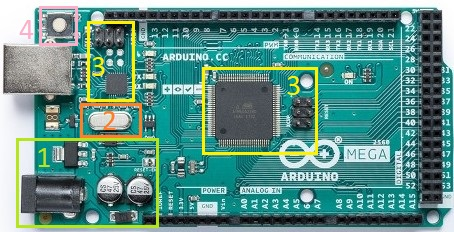
\includegraphics[scale=0.6]{figures/top}
		
			\caption{Top view of the Arduino MEGA 2560 REV3 board\cite{arduino}}
	
	\end{figure}
\end{center}


%--------------------------------------------------------------------------------------

\section{Power Regulator Circuit}

Power regular circuit is used to regulate the input voltage of the board form a voltage in range of 7V-12V to lower +5V, as this is the operating voltage of the Arduino MEGA board.It consists of following electronic components.

\begin{center}
	\begin{figure}[!h]
		\centering
		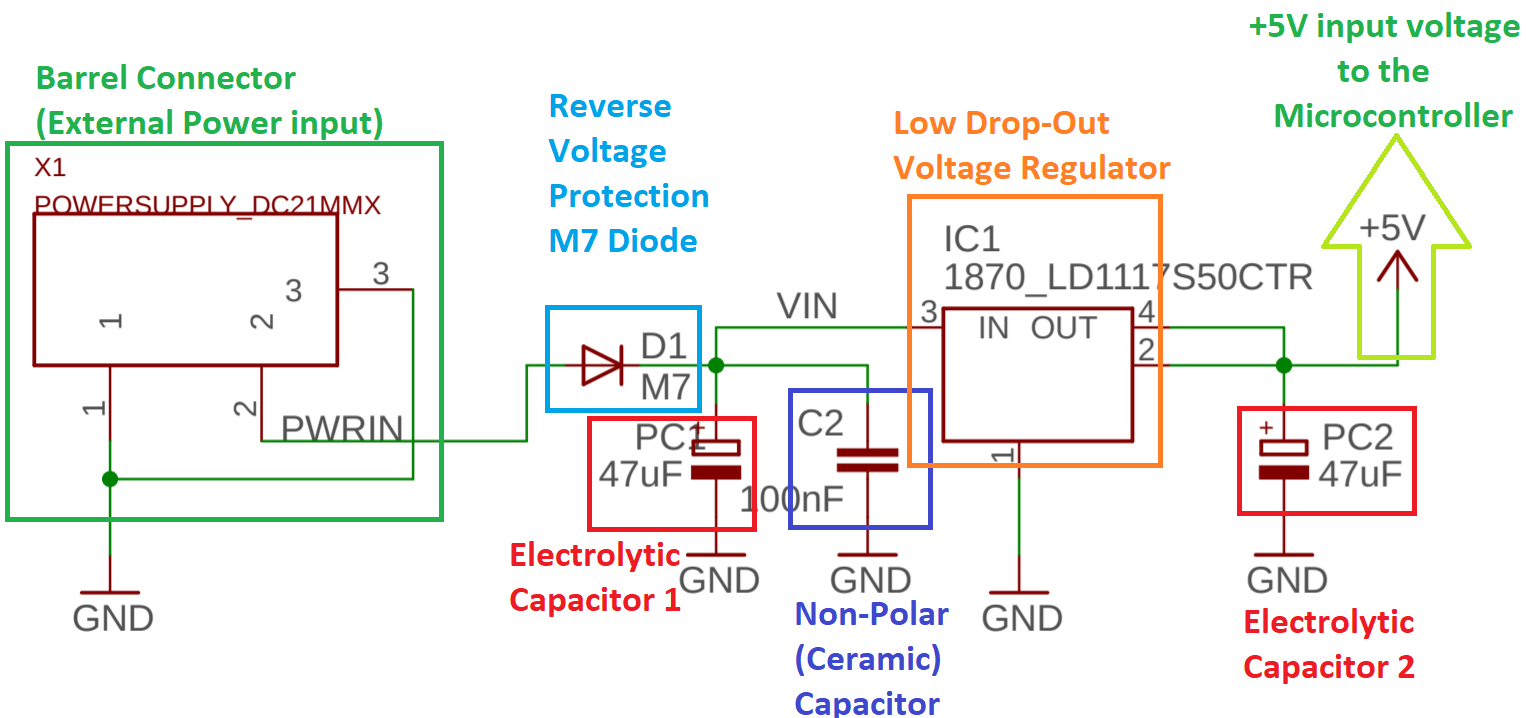
\includegraphics[scale=0.3]{figures/vreg}
		\caption{Power regulator schematic diagram\cite{arduino}}
	\end{figure}
\end{center}


\subsection{Barrel connector}

This barrel type connector is used to supply DC power (\textit{6V-12V is recommended}) to the board from an external power source.

\subsection{Reverse Voltage Protection Diode}

If the polarity of input supply voltage is accidentally reversed the board may get damaged. This M7 diode (\textit{SMD version of 1N4007 diode}) provides the protection at such situations. 

\subsection{Electrolytic Capacitors}

Polarized capacitors are used to reduce  possible small fluctuations(electrical noise) in the input voltage/current. Capacitors with fairly high capacitance (47$\mu$F) is used for this purpose as they can store high electric charge.

\subsection{Non-polarized Capacitors}

Although electrolytic capacitors have high capacitance it is considerably slow in discharging process due to its high series resistance (capacitive reactance). As a solution for this draw back,electrolytic capacitor is discharged through a  non-polar capacitor with very low capacitance(100nF) and an extremely small discharging time.

\subsection{LD1117S50CTR Voltage Regulator IC}

This IC continues to work although the input voltage is very close to the required output, and able to handle currents up to 800 mA. Also it can regulate voltages in the range 6.5V to 15V to lower 5V level\cite{lowdrop}.


\section{Clock Circuit}


Micro-controllers use clock signal to trigger events and keep track of time as everything happens with respect to time. clock Circuitry is responsible of  generating this clock signal which is basically an electronic signal periodically toggle between two states like a Square wave\cite{osci}. 

\begin{center}
	\begin{figure}[!h]
		\centering
		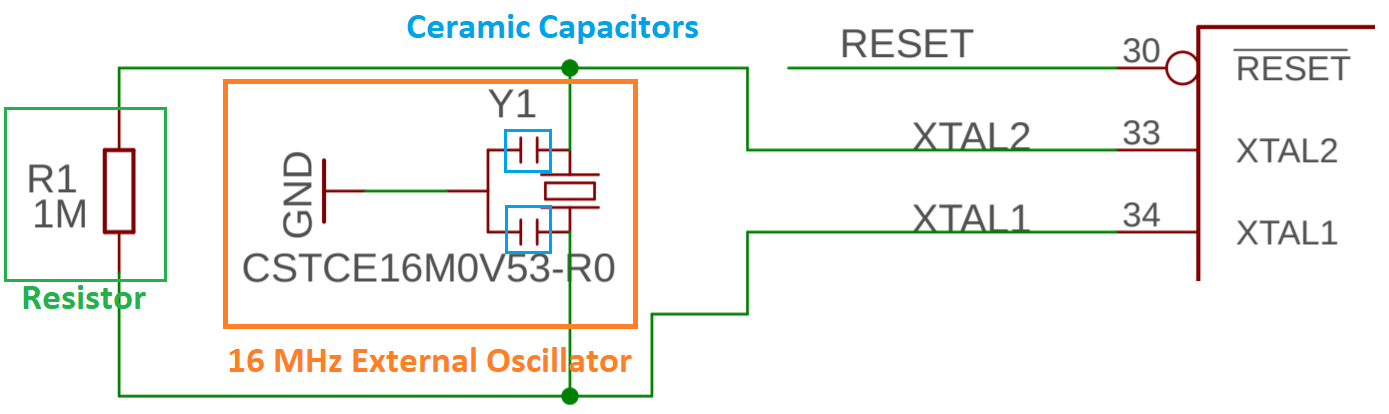
\includegraphics[scale=0.3]{figures/clock}
		\caption{External oscillator schematic diagram\cite{arduino}}
	\end{figure}
\end{center}

\subsection{Crystal Oscillator}

Arduino MEGA 2560 uses 16 MHz oscillator to generate this clock signal. It consists of a \textit{piezoelectric Crystal resonator}\cite{crystal} and two ceramic capacitors in order to adjust resonance frequency. 

 
\section{In-system Programming/ In-circuit Serial Programming Circuit}

Arduino MEGA2560 board has two ICSP headers named as ICSP1 and ICSP. Both headers have 6 pins and are arranged in 2 * 3 arrays. 6 pins are named as MISO, MOSI, SCK, V+(+5V), Ground, and Reset\cite{icsp}.

\begin{center}
	\begin{figure}[!h]
		\centering
		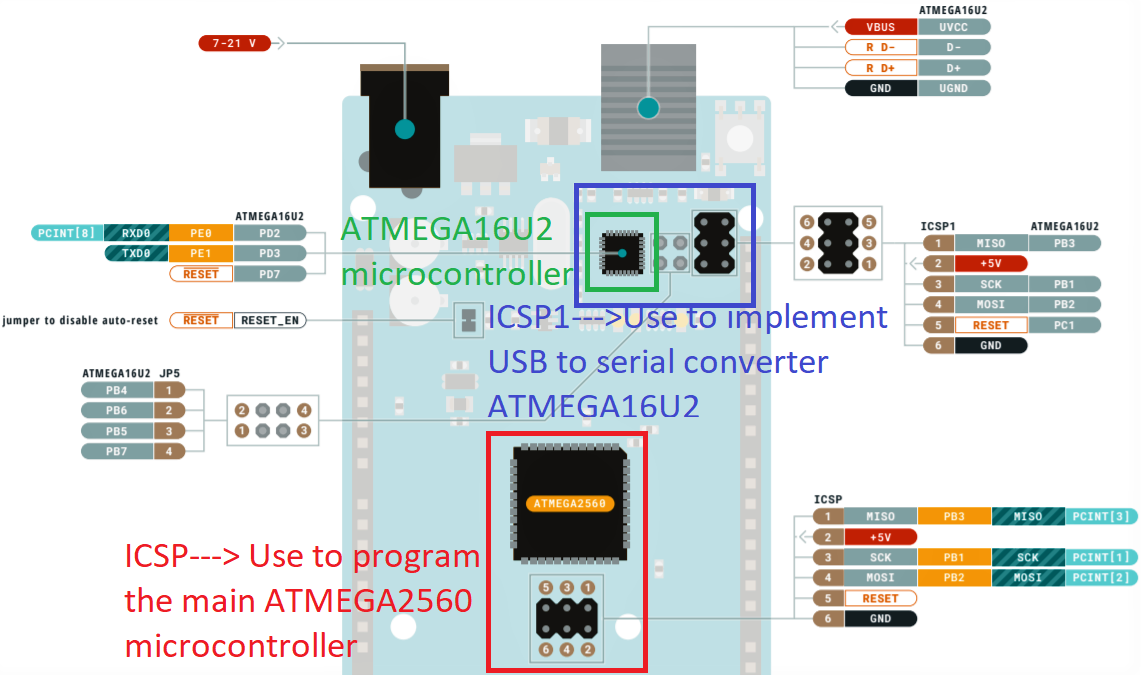
\includegraphics[scale=0.35]{figures/programmer}
		\caption{ICSP headers in an Arduino MEGA2560 board\cite{arduino}}
	\end{figure}
\end{center}

\subsection{ATMEGA16U2 microcontroller}

Programs related to USB to serial conversion are stored here. This supports to upload the programs into  main ATMEGA2560 microcontroller, simply through  the USB cable.

\subsection{ICSP1}

ICSP1 header is used to implement the USB to serial converter micro-controller(\textit{ATMEGA16U2}).

\subsection{ICSP}  

ICSP header is used to directly program the main microcontroller of the Arduino MEGA2560 board, whenever the USB to serial converter can not be used to program the microcontroller due to any failure of converter. To do this additional ISP/ICSP programmer(\textit{an electronic circuitry}) is needed.

\section{Reset Circuit}
There are two mechanisms  to reset the Arduino MEGA2560 board. One of them is manual while the other one is done by the USB to serial converter chip. Here the reset pin is \textit{active low}, i.e. microcontroller get reset whenever the  pin receives a low state signal. 

\subsection{Manual Method}

To reset the microcontroller there is a TS42 type press button switch on the board. When it is pressed, reset pin is grounded. This process resets the microcontroller.

\begin{center}
	\begin{figure}[!h]
		\centering
		\includegraphics[scale=0.5]{figures/capture}
		\caption{Manual resetting\cite{arduino}}
	\end{figure}
\end{center}




\subsection{Reset through the ATMEGA16U2}

In this method microcontroller get reset whenever a connection is made with the Arduino IDE through its USB cable. The required DTR(Data Terminal Ready)signal is sent by the ATMEGA16U2 to the RESET pin of the ATMEGA2560 at the beginning of each connecting.
\begin{center}
	\begin{figure}[!h]
		\centering
		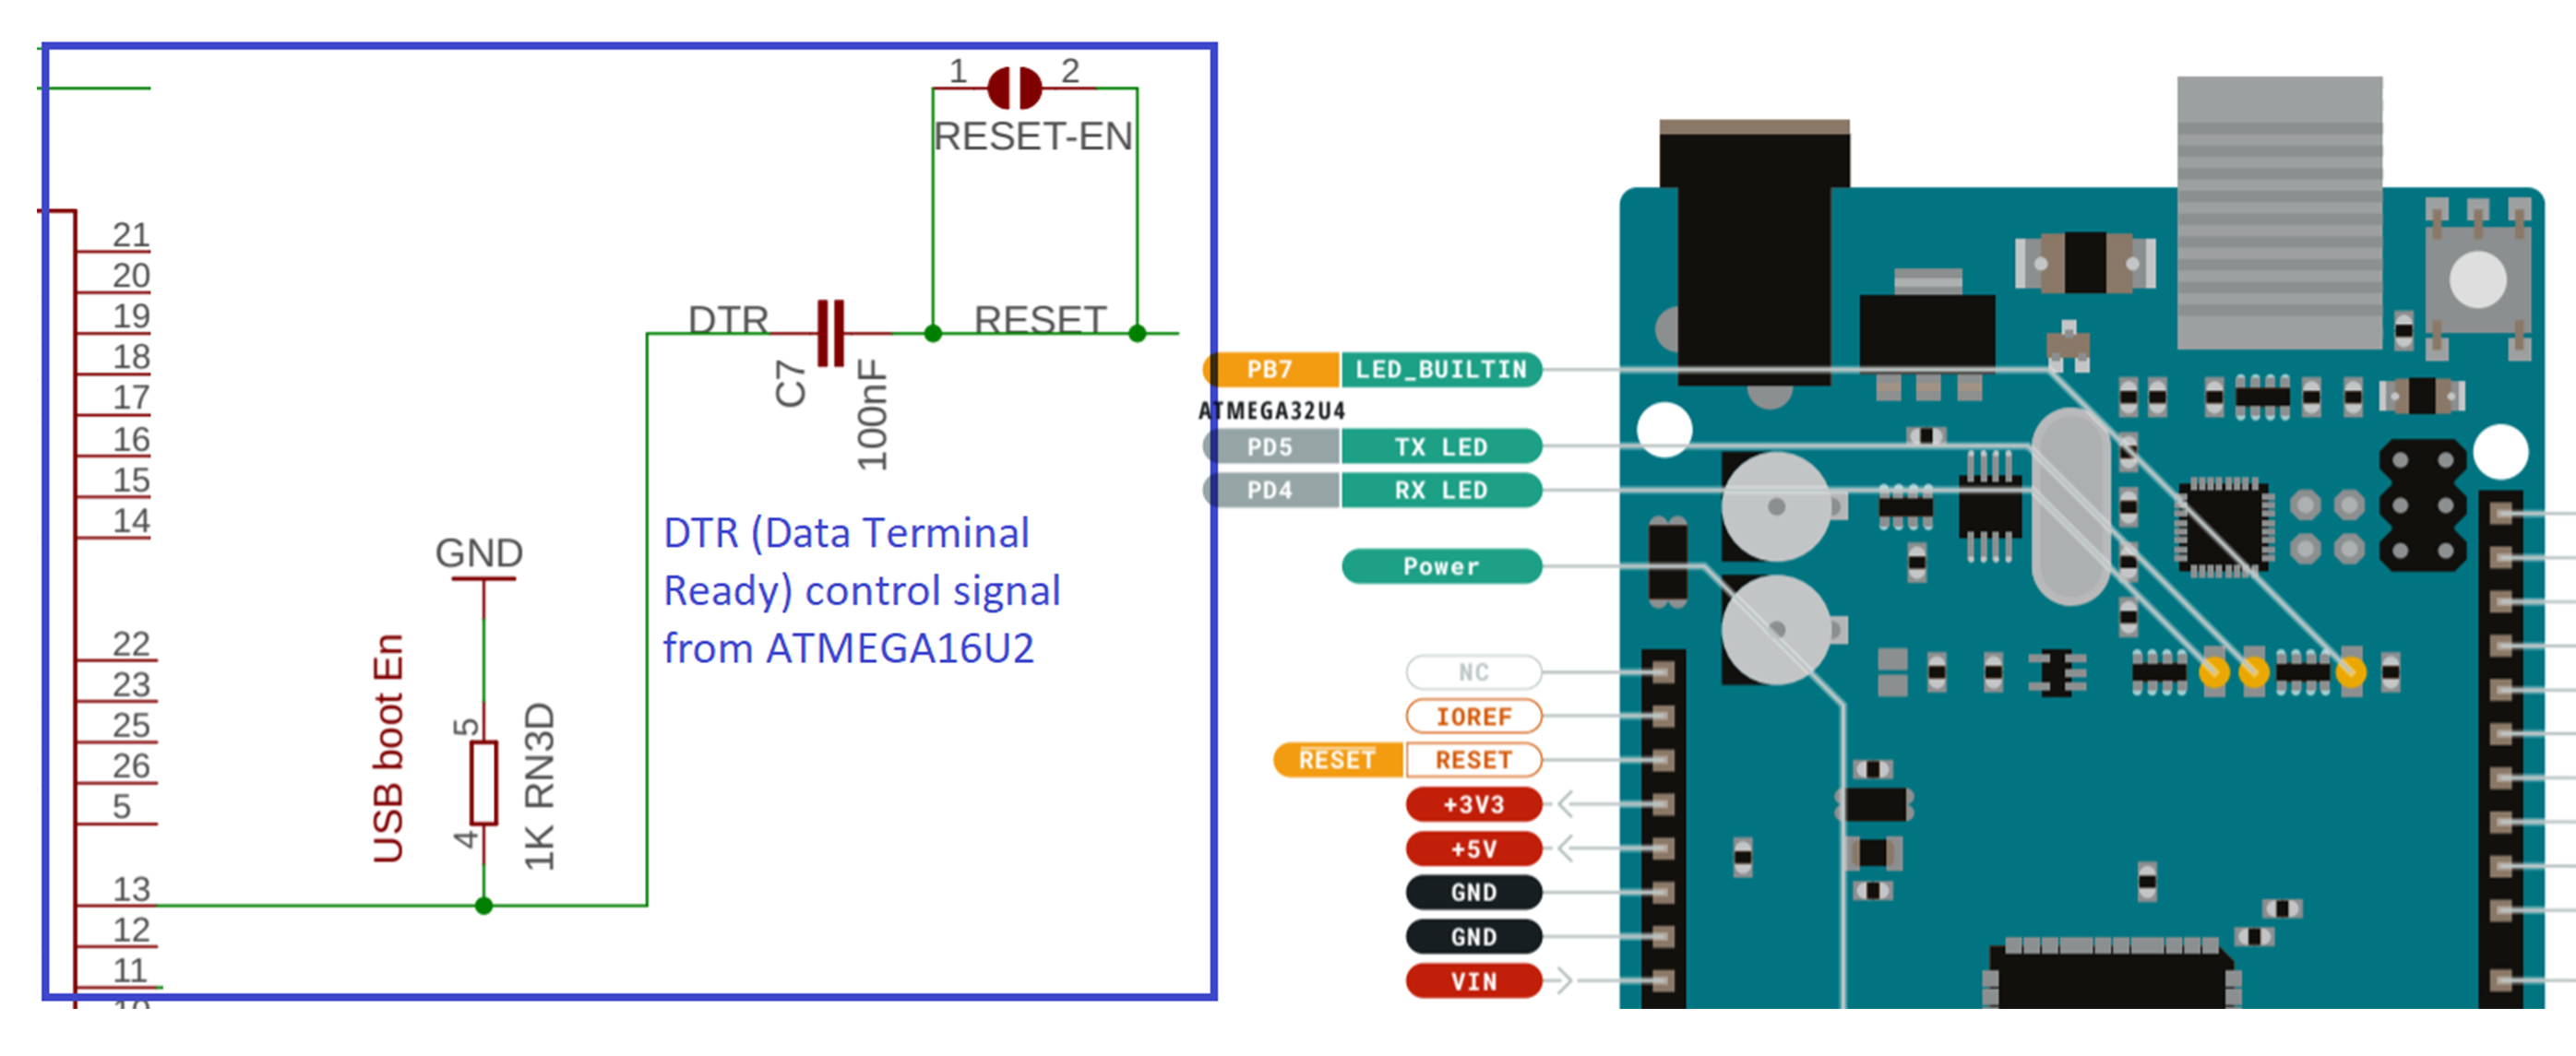
\includegraphics[scale=0.3]{figures/SOFT}
		\caption{Automatic resetting\cite{arduino}}
	\end{figure}
\end{center}


{\scriptsize
\bibliographystyle{plain}
\bibliography{reference} }	
\end{document}